\chapter{The FETI formulation}\label{cha:feti_formulation}
\section{Problem Setup}
The reference problem for all further considerations is described in Figure~\ref{fig:reference_problem}. For the sake of simplicity, a two domain setup shall be considered here, a generalization to an arbitrary number of sub-domains can, however easily be derived.


\begin{figure}[h]
  \centering
  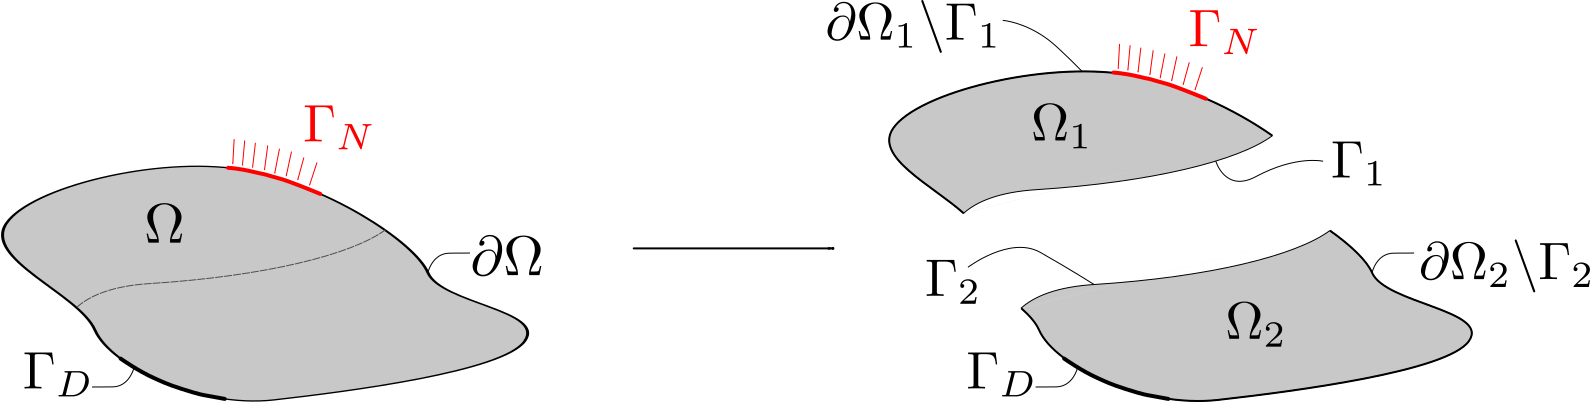
\includegraphics[width=0.8\textwidth]{./fig/eps/drawing1}
  \caption[Domain decomposition reference problem]{Reference problem. The simple case of two substructures is considered here, a generalization to an arbirtray number of substructures can, however, be easily achieved. The domain $\Omega$ is split into the subdomains $\domainone$ and $\domaintwo$ by the interface $\Gamma$. The aim of all DD methods is to distribute those domains to different proccessing nodes and solve the problems as locally as possible. Of course, some interprocessor communication can not be avoided, since information(e.g. the boundary conditions) has to be propagated from one domain to the other. Looking at this example it shall also be noted, that substructuring may introduce so-called "floating substructures", which means substructures can have rigid body modes, although the overall system does not.}\label{fig:reference_problem}
\end{figure}
\begin{figure}[h!]
  \begin{center}
    \includestandalone{\tikzpath/setup_quad4_basic_example}
    \caption[Simple discretized problem]{Basic discretized problem. The setup consists of four substructures, each of which is built up of just one quadrilateral element. Albeit very simple, this example can be used to explain all relevant operators and problems concerning the FETI method. The element/node/dof/Lagrange-multiplier numbering scheme is consistent with the Matlab code developed for this thesis~\cite{FEMAC}. Its is very crucial to note the difference between the global numbering scheme and the substructure-based numbering scheme. }
    \label{fig:simple_discretized_example}
  \end{center}
\end{figure}

\begin{figure}[h!]
  \begin{center}
    \includestandalone{\tikzpath/setup_quad4_basic_example_sub3}
    \caption[Simple discretized problem - detail substructure 3]{Detailed view of the bottom right substructure. Substructure-local dof indices are printed here, since they are used to create the assembly operator $\asmop$. For this particular example, the assembly and trace operator of the bottom right substructure are given in Equation~\eqref{eq:asmop_and_traceop_example}.}
    \label{fig:simple_discretized_example_detail_sub}
  \end{center}
\end{figure}



\section{General}

The simple problem of linear elasticity can be formulated in $\Omega$ as:
\begin{align}
  \dmat{K}\dvec{u}=\dvec{f} 
\end{align}
\\
The FETI-method tears the domain apart, introducing two sub-domains. Thus, a compatibility condition has to be imposed, linking them together. The FETI method enforces this compatibility by the Lagrange multiplier approach(see Section~\ref{sec:lagrange_multiplier_approach}). One can thus write:
\begin{align}
  \idone{\dmat K}\idone{\dvec u}                   & =\idone{\dvec f}\label{eq:elasticity_equation_domain1} \\
  \idtwo{\dmat K}\idtwo{\dvec u}                   & =\idtwo{\dvec f}\label{eq:elasticity_equation_domain2} \\
  (\dvec{\lambda},\dvec{\idtwo u}-\dvec{\idone u}) & =0\label{eq:compatibility_constraint}                  
\end{align}
\\
In contrast to e.g. the mortar method, the FETI approach, enforces Equation~\eqref{eq:compatibility_constraint} not in an integral, but in a point-wise sense. This does not introduce errors, since only conforming meshes are considered here.\\
For an arbitrary number of sub-domains Equations~\eqref{eq:elasticity_equation_domain1}-\eqref{eq:compatibility_constraint} can be equivalently formulated as
\begin{align}
  \ids{\stiffmat} \ids{\dispvec} = \ids{\dvec{f}}+{\ids{\traceop}}^T {\ids{\asmop}}^T \lagvec\label{eq:basic_subdomain_equation} \\
  \sum_s \ids{\traceop} \ids{\asmop} \ids{\dispvec}=0\label{eq:basic_subdomain_equation_asm}                                     
\end{align}
where $\ids{\asmop}$ is a substructure-based, boolean assembly operator, who's rows correspond to the global Lagrange multipliers, and who's columns relate to the substructure-based interface-dofs. A negative sign is used, when the Lagrange multiplier connects to a substructure with a smaller ID, otherwise a positive sign is entered. This reflects the condition from Equation~\eqref{eq:compatibility_constraint}.\\
The trace operators $\ids{\traceop}$, map the columns of $\ids{\asmop}$ to a substructure-based total dof numbering scheme.
\\
For the basic example as described in Figure~\ref{fig:simple_discretized_example} the operators $\asmop$ and $\traceop$ for the bottom left substructure(isolated in Figure~\ref{fig:simple_discretized_example_detail_sub}) are given as

\begin{equation}
  \begin{array}{lc}
    \texttt{$B^{(3)}=$} & \kbordermatrix{\text{} & 1 & 2 & 3 & 4 & 5 & 6\cr 
    1&\0&\0&\0&\0&\0&\0\cr
    2&\0&\0&\0&\0&\0&\0\cr
    3&\0&\0&\0&\0&\0&\0\cr
    4&\0&\0&\0&\0&\0&\0\cr
    5&\0&\0&-1&\0&\0&\0\cr
    6&\0&\0&\0&-1&\0&\0\cr
    7&\0&\0&\0&\0&\0&\0\cr
    8&\0&\0&\0&\0&\0&\0\cr
    9&\0&\0&\0&\0&\0&\0\cr
    10&\0&\0&\0&\0&\0&\0\cr
    11&\0&\0&-1&\0&\0&\0\cr
    12&\0&\0&\0&-1&\0&\0\cr
    13&\0&\0&\0&\0&-1&\0\cr
    14&\0&\0&\0&\0&\0&-1\cr
    15&\0&\0&\0&\0&\0&\0\cr
    16&\0&\0&\0&\0&\0&\0\cr
    17&1&\0&\0&\0&\0&\0\cr
    18&\0&1&\0&\0&\0&\0\cr
    19&\0&\0&1&\0&\0&\0\cr
    20&\0&\0&\0&1&\0&\0}\\
  \end{array},~~
  \begin{array}{lc}
    \texttt{$\traceop^{(3)}=$} & \kbordermatrix{\text{} & 1 & 2 & 3 & 4 & 5 & 6 & 7 & 8\cr 
    1&1&\0&\0&\0&\0&\0&\0&\0\cr
    2&\0&1&\0&\0&\0&\0&\0&\0\cr
    3&\0&\0&\0&\0&1&\0&\0&\0\cr
    4&\0&\0&\0&\0&\0&1&\0&\0\cr
    5&\0&\0&\0&\0&\0&\0&1&\0\cr
    6&\0&\0&\0&\0&\0&\0&\0&1}\\
  \end{array}
  \label{eq:asmop_and_traceop_example}
\end{equation}
\\
The basic idea of FETI now is to reduce the substructure domain problems to a connected interface problem. This can be achieved very elegantly, by rearranging the basic equations \eqref{eq:basic_subdomain_equation}-\eqref{eq:basic_subdomain_equation_asm} and was first described in~\cite{Farhat1991}.
\\
One  should note, that a solution to Equation~\eqref{eq:basic_subdomain_equation} can only exist if $(\ids{\dvec{f}}+{\ids{\traceop}}^T {\ids{\asmop}}^T \lagvec)$ is orthogonal to the null-space of $\stiffmat$.
\\
\section{Interface reduction}\label{sec:interface_reduction}
As mentioned FETI is a reduction technique that solves for the interface unknowns only. After the interface solution has been obtained, the global solution will be recovered.\\
This section is denoted to an step by step explanation of the reduction and subsequent recovery process. We will end up with a system of Equations in the interface unknowns(ans possibly some rigid body modes) only. The process of solving that system will be discussed in Section~\ref{cha:feti_solvers}.
\\
\\
We begin considerations by a reformulation of Equation\eqref{eq:basic_subdomain_equation} as:
\begin{align}
  \ids{\dispvec}=\inv{\ids{\stiffmat}} (\ids{\dvec{f}}+\tp{\ids{\traceop}} \tp{\ids{\asmop}} \lagvec) 
  \label{eq:displacement_recovery}                                                                    
\end{align}
However, as will be explained in Section~\ref{sec:natural_subspace}, for static problems it is required to search for $\lagvec$ in the so-called natural subspace, which is is the rigid body mode free space. Thus,
\begin{align}
  \ids{\dispvec}=\inv{\ids{\stiffmat}} (\ids{\dvec{f}}+\tp{\ids{\traceop}} \tp{\ids{\asmop}} \lagvec) + \ids{\nullspacemat} \ids{\rmodevec} 
  \label{eq:interpolation_full_displacement}                                                                                                
\end{align}
where $\ids{\nullspacemat}$ denotes the nullspace of $\ids{\stiffmat}$ and $\ids{\rmodevec}$ are the generalized coordinates for the interpolation. It should be noted that for the iterative solution process that will follow, a practical implementation will involve a matrix factorization anyway. The nullspace thus comes as a by-product for free.
\\
\\
Inserting Equation~\eqref{eq:interpolation_full_displacement} into Equation~\eqref{eq:basic_subdomain_equation_asm} gives
\begin{align}
    & \sum_s \ids{\asmop} \ids{\traceop} \big(\inv{\ids{\stiffmat}} (\ids{\dvec{f}}+\tp{\ids{\traceop}} \tp{\ids{\asmop}} \lagvec)+\nullspacemat\ids{\rmodevec}\big)=0\text{   or} \\
    & \underbrace{(\sum_s \underbrace{ \ids{\asmop}                                                                                                                                             
  \underbrace{\ids{\traceop} \inv{\ids{\stiffmat}} \tp{\ids{\traceop}}}_{\ids{\dmat{F}}}
  \tp{\ids{\asmop}} }_{\asmids{\locdualschur}} }_{\dmat{F}} ) \lagvec +
  \sum_s \underbrace{\ids{\asmop}  \ids{\traceop} \ids{\nullspacemat}}_{\ids{\rmodespace}} \ids{\rmodevec}
  =
  \underbrace{\sum_s \ids{\asmop}  \ids{\traceop} \inv{\ids{\stiffmat}}  \ids{\forcevec}}_{-\dvec{d}}
\end{align}
\\
where the abbreviations $\ids{\locdualschur}$ for the local dual schur complement, $\asmids{\locdualschur}$ for the assembled local dual schur complement, $\rmodespace$ for the rigid body mode space and $\ifacedispvec$ for the condensed interface displacements have been introduced.\\
\\
So far, the system is under-determined, since we only have two equations, but three unknowns. However, a third equation can be derived by looking at Equation~\ref{eq:basic_subdomain_equation}. If $\ids{\stiffmat}$ is singular, a solution can only exist if $(\ids{\dvec{f}}+{\ids{\traceop}}^T {\ids{\asmop}}^T \lagvec)$ has no component in the Nullspace $\nullspacemat$:
\begin{align}
    & \tp{\ids{\nullspacemat}}(\ids{\dvec{f}}+{\ids{\traceop}}^T {\ids{\asmop}}^T \lagvec)=0\text{  or}\label{eq:reason_natural_subspace} \\
    & \underbrace{\tp{\ids{\nullspacemat}} \ids{\dvec{f}}}_{\tp{\ids{\dvec{e}}}} =                                                        
  \underbrace{\tp{\ids{\nullspacemat}}  \tp{\ids{\traceop}} \tp{\ids{\asmop}}}_{\tp{\ids{\rmodespace}}} \lagvec  
\end{align}
where the abbreviation $\dvec{e}$ for the components of the external forces in the rigid body mode space has been established.
\\
Moreover, we can introduce
\begin{align}
  \ids{\locschur}&=\ids{\stiffmat_{bb}}-\ids{\stiffmat_{bi}}\pinv{\ids{\stiffmat_{ii}}}\ids{\stiffmat_{ib}}\label{eq:locschur} \\
  \asmids{\locschur}&=\tp{\asmop} \left( \ids{\locschur} \right) \asmop \\
  \locschur&= \sum_s \asmids{\locschur}
\end{align}
as the local schur operator, assembled local schur operator and global schur operator respectively.\\
Throughout this thesis $\ids{(\cdot)}$ will be used for substructure local quantities and $\asmids{(\cdot)}=\sum_s \ids{\asmop}\ids{\traceop} \ids{(\cdot)} \tp{\ids{\traceop}} \tp{\ids{\asmop}}$ denotes the assembled local quantity.

\section{Matrix notation}\label{sec:matrix_notation}
Putting all previously derived Equations together, one can finally write the basic FETI Problem in matrix notation as:
\begin{align}
  \begin{bmatrix}
  \locdualschur    & \rmodespace \\
  \tp{\rmodespace} & \dmat{0}    
  \end{bmatrix}
  \begin{bmatrix}
  \lagvec\\
  \rmodevec
  \end{bmatrix}
  =
  \begin{bmatrix}
  \ifacedispvec\\
  \dvec{e}
  \end{bmatrix}
  \label{eq:feti_equation_system}
\end{align}
\\
Where
\begin{align}
  %\ids{\nullspacemat}&=ker(\ids{\stiffmat}) \\
  \dmat{e}      & =\tp{\begin{bmatrix} \cdots,\tp{\ids{\forcevec}} \ids{\nullspacemat},\cdots \end{bmatrix}}   \\
  \rmodespace   & =\begin{bmatrix} \cdots,\ids{\asmop}\ids{\traceop}\ids{\nullspacemat},\cdots \end{bmatrix}   \\
  \locdualschur & =~~\sum_s \ids{\asmop} \ids{\locdualschur} \tp{\ids{\asmop}} \label{eq:definition_dualschur} \\
  \ifacedispvec & =-\sum_s \ids{\asmop}  \ids{\traceop} \inv{\ids{\stiffmat}}  \ids{\forcevec}                 
\end{align}
and $\lagvec$ are the unknown interface forces, $\rmodevec$ the rigid body mode components respectively.
\\
\section{The natural subspace}\label{sec:natural_subspace}
As was explained in \eqref{eq:reason_natural_subspace}, classical FETI formulation encounters a problem for static calculations if the local stiffness matrix is singular. In that case, we required
\begin{align}
    & \tp{\ids{\nullspacemat}}(\ids{\dvec{f}}+{\ids{\traceop}}^T {\ids{\asmop}}^T \lagvec)=\dvec{0}%\label{eq:reason_natural_subspace} 
\end{align}
where $\asmop$ is the substructure based boolean assembly operator, introduced in Equation~\eqref{eq:basic_subdomain_equation}, consisting of $0,+1,-1$, defined such that the continuity conditions for each Lagrange multiplier is ensured(see~Equation~\eqref{eq:compatibility_constraint})
\\
We had solved this problem by prescribing the
\begin{align}
  \tp{\rmodespace} \totalgap_i =0           
  \label{eq:orthogonality_natural_subspace} 
\end{align}
\\
Inserting Equation~\eqref{eq:totalgap} one can thus write
\begin{align}
  \tp{\rmodespace} (\ifacedispvec-\locdualschur \lagvec_i - \rmodespace \rmodevec_i ) =0 
\end{align}
\\
which can easily be reformulated to
\begin{align}
  \tp{\rmodespace} \underbrace{(\ifacedispvec- \locdualschur \lagvec_i)}_{\resvec_i} - \tp{\rmodespace} \rmodespace \rmodevec_i =0 
\end{align}
\\
Solved for $\rmodevec_i$ this gives
\begin{align}
  \rmodevec_i=\inv{(\tp{\rmodespace}\rmodespace)}\tp{\rmodespace}\resvec_i 
  \label{eq:r_to_alpha}                                                    
\end{align}
\\
Inserting Equation~\eqref{eq:r_to_alpha} into Equation~\eqref{eq:totalgap} gives
\begin{align}
  \totalgap_i & =\resvec_i-\rmodespace \inv{(\tp{\rmodespace}\rmodespace)}\tp{\rmodespace}\resvec_i                       \\
              & =\underbrace{(\eyemat-\rmodespace \inv{(\tp{\rmodespace}\rmodespace)}\tp{\rmodespace})}_{\projn}\resvec_i 
\end{align}
where by looking at the equation, $\projn$ can be interpreted as a projection operator, that removes all rigid body components from $\resvec_i$.
\\
As first described in \cite{Farhat1992}, and further investigated in \cite{RixenPhD} it is often advantageous to choose $\totalgap_i$ to be not simply orthogonal, but A-orthogonal to a matrix A:
\begin{align}
  \tp{\rmodespace} \scalemat \totalgap_i =0 
\end{align}
\\
which leads to the following expression for the natural subspace projector
\begin{align}
  \tp{\projn}=\eyemat-\scalemat\rmodespace \inv{(\tp{\rmodespace}\scalemat\rmodespace)}\tp{\rmodespace} 
\end{align}

\paragraph{Choices for $\dmat{A}$}
The equation for the natural subspace projector above has introduced the matrix $\scalemat$. It has been shown in\cite{RixenPhD} that this matrix plays the role of a preconditioner for the coarse grid displacements.
Ideally, the preconditioner used for the Conjugate Gradient iterations should be taken for $\scalemat$.
\\
The Equations in the previous chapter show that the Lagrange multipliers are corrected by a step of $\scalemat \rmodespace$ at every Conjugate Gradient iteration.
From a dimensional point of view, one can thus argue that since $\rmodespace$ represents restrictions on the displacement modes, $\scalemat$ should represent a stiffness matrix. Particularly, since the product represents interface forces due to rigid body modes, the ideal choice for $\scalemat$ is the preconditioner.\\
However, choosing the preconditioner typically introduces a significant fill-in in the inversion of $\rmodespace \scalemat \tp{\rmodespace}$.\\
The bottom line is that in most cases simply choosing $\scalemat=\eyemat$ is the more efficient option. During this thesis, this choice has been retained.

\section{Residuum formulation}\label{sec:residuum_formulation}
The natural solver choice for the FETI problem is the Conjugate Gradient method. This chapter aims at formulating the CG algorithm specifically for the FETI problem. Some alternations to the classical CG notation will be done to ensure parallel efficiency of the method.\\
\\
The CG algorithm consists of three main points. Firstly new search directions are created, these search directions are then updated through orthogonalization to the previous one, and finally an optimal step length is determined by minimizing the residual error along this direction. In practice, Orthogonalization is performed with regards to all previous search directions due to the finite precision of the machine.
\\
The first question is therefore, how to derive the search directions. Since FETI operates on interface forces as primary variables, we need an update for the force vector.
\\
For any given approximation $\lagvec$ to the interface force solution one can calculate the resulting gap between the substructures as
\begin{align}
  \totalgap_i=\sum_s \ids{\asmop}\ids{\dispvec}=\ifacedispvec-\locdualschur \lagvec_i - \rmodespace \rmodevec = \dvec{0} \label{eq:totalgap} 
\end{align}
\\
The gap, projected to the natural subspace can thus be written as
\begin{align}
  \resvec_i=\tp{\projn}(\ifacedispvec-\locdualschur\lagnvec_i) 
\end{align}
where the rigid body mode component vanished due to the very definition of the natural subspace projector $\projn$.
\\
The idea now it to estimate the interface forces associated with displacement of that value by a preconditioning step:
\begin{align}
  \dvec{z}_i=\scaled{\locschur}\resvec_i 
\end{align}
\\
Since the local schur operator has full rank, one again need a projection to the natural subspace to eliminate all rigid body mode components.
\begin{align}
  \dvec{w}_i=\projn\dvec{z}_i 
\end{align}
\\

The dual schur operator $\locdualschur$ is used to calculate the interface displacements related to this forces as
\begin{align}
\dvec{q}_i = \locdualschur \sdirnspace_i
\end{align}


After full orthogonalization of the search direction a line-search is performed to minimize the energy expression. The Lagrange multiplier is then updated as

\begin{align}
\delta_i&=\tp{\dvec{q}_i}\dvec{w}_i\\
\gamma_i&=\tp{\dvec{r}_i} \dvec{z}_i\\
\lagfvec_{i+1}&=\lagfvec_i+(\gamma_i/\delta_i)\sdirnspace_i 
\end{align}
\\
The resulting gap to to the updated force does not need to be explicitly computed, but instead it can be updated too as

\begin{align}
  \resvec_{i+1}=\resvec_i-(\gamma_i/\delta_i)\tp{\projn}\sdirnspacecspace_i 
\end{align}
\\
The process is then repeated until satisfying convergence has been obtained.
The full solution for lambda is then recovered as
\begin{align}
  \lagvec=\lagvec_0+\lambda_ F 
\end{align}
The displacements can finally be recovered by Equation~\eqref{eq:displacement_recovery}.

\section{Preconditioners}\label{sec:precond}
As will be explained in Chapter~\ref{cha:iterative_solvers}, iterative solution techniques typically use preconditioners to accelerate convergence.
As can be seen from the formulation above preconditioner in the context of FETI is an approximation to the operator
\begin{align}
\sum_s \ids{\asmop} \inv{\ids{\stiffmat}} \tp{\ids{\asmop}}
\end{align}
The natural choice for this problem in the FETI formulation can be identified as
\begin{align}
\inv{\precond}=\sum_s \ids{\asmop} \ids{\traceop} \ids{\locschur} \tp{\ids{\traceop}} \tp{\ids{\asmop}}
\end{align}
where the schur complement $\locschur$ is defined as
\begin{align}
\ids{\locschur}=\ids{\stiffmat}_{bb}-\ids{\stiffmat}_{bi} \pinv{\ids{\stiffmat}_{ii}} \ids{\stiffmat}_{ib}
\label{eq:locschur2}
\end{align}
This version of the preconditioner is typically denoted as Dirichlet preconditioner in the literature.\\
The pseudo inversion of $\pinv{\ids{\stiffmat}}$ is costly and introduces a lot of non-zero entries in the preconditioner matrix. Therefore~\cite{Farhat1991} proposed to neglect the second term in Equation~\eqref{eq:locschur2}, which results in the o called lumped preconditioner. One can summarize
\begin{align}
\inv{\precond}_D&=\sum_s \ids{\asmop} \ids{\traceop}
\left(  \ids{\stiffmat}_{bb}-\ids{\stiffmat}_{bi} \pinv{\ids{\stiffmat}_{ii}} \ids{\stiffmat}_{ib}  \right)
\tp{\ids{\traceop}} \tp{\ids{\asmop}} &\text{ ... Dirichlet Preconditioner} \\
\inv{\precond}_L&=\sum_s \ids{\asmop} \ids{\traceop}
\pinv{\ids{\stiffmat}_{ii}}
\tp{\ids{\traceop}} \tp{\ids{\asmop}} &\text{ ... Lumped Preconditioner}
\label{eq:precond}
\end{align}
However, this definition of the preconditioner has been shown to be not consistent in~\cite{Rixen1999a} for the case where crosspoints are present. A Crosspoint is a point, of the mesh where more than two substructures meet. An example would be node 5 in Figure~\ref{fig:simple_discretized_example} where all four substructures meet. It is obvious that our definition of the Lagrange multipliers introduces a redundancy in the Equations, since one could simply drop the four diagonal Lagrange multipliers, and still the problem would be fully determined. The identifications and removal of redundant Lagrange multipliers, however, is cumbersome and inefficient.\\
From a mechanical point of view, the problem arises when updating the interface displacements in the Conjugate Gradient. If one dof carries more than one Lagrange multiplier, than its displacement is multiply updated and the update steps typically contradict on another in a non-converged situation.\\
A simple and effective approach to eliminates this problem is Multiplicity Scaling. It can be formulated as
\begin{align}
\inv{\precond}_{D}&=\sum_s \ids{\dmat{D}} \ids{\asmop} \ids{\traceop}
\ids{\locschur}
\tp{\ids{\traceop}} \tp{\ids{\asmop}} \ids{\dmat{D}} &\text{ ... Dirichlet Preconditioner} \\
\inv{\precond}_{L}&=\sum_s \ids{\dmat{D}}  \ids{\asmop} \ids{\traceop}
\pinv{\ids{\stiffmat}_{ii}}
\tp{\ids{\traceop}} \tp{\ids{\asmop}} \ids{\dmat{D}}  &\text{ ... Lumped Preconditioner}
\label{eq:precond_mscaled}
\end{align}
where $\ids{\dmat{D}}$ is a substructure based diagonal scaling matrix, that holds the multiplicity of the corresponding interface dofs. As multiplicity of a dof we define the number of Lagrange multiplier related to that dof. This multiplicity can be derived very elegantly as
\begin{align}
\dmat{D}&=\frac{1}{2} \tp{\asmop}\asmop\\
\asmop&=\sum_s \ids{\asmop} \ids{\traceop}
\end{align}
\\
Another inconsistency, when it comes to preconditioners are heterogeneities across substructure interfaces. Similarly to the considerations above, a scaling approach can be defined too, according to

\begin{align}
\inv{\precond}_{D}&=\sum_s \ids{\dmat{\beta}} \ids{\asmop} \ids{\traceop}
\ids{\locschur}
\tp{\ids{\traceop}} \tp{\ids{\asmop}} \ids{\dmat{\beta}} &\text{ ... Dirichlet Preconditioner} \\
\inv{\precond}_{L}&=\sum_s \ids{\dmat{\beta}}  \ids{\asmop} \ids{\traceop}
\pinv{\ids{\stiffmat}_{ii}}
\tp{\ids{\traceop}} \tp{\ids{\asmop}} \ids{\dmat{\beta}}  &\text{ ... Lumped Preconditioner} \\
\beta^{(s),i} &= diag(\stiffmat_{bb}^{(s),i}) \left[  \sum_{r:\Gamma_I^i \subset \{  \Gamma_I \cap \Gamma_I^{(r)}  \} } diag(\stiffmat_{bb}^{(r),i})  \right]^{-1} &
\label{eq:precond_kscaled}
\end{align}
Rixen and Farhat introduced this approach as "Superlumped Smoothed Preconditioner". In the literature the more descriptive term "K-scaling" is often used.\\
Both scaling approaches introduced here are appealing since they do not introduce a significant extra cost, while drastically improving the solver performance, especially for the case with high heterogeneities across the interface. The policy in this thesis, that can also be recommended with clear considence as a standard approach, therefore is to always use both of these scaling types combined. Exceptions(see Chapter~\ref{cha:numerical_assesment}) will be explicitly mentioned.


\section{Scalability}\label{sec:scalability}
The main goal of a DD algorithm is scalability. Generally, one can distinguish numerical scalability and parallel scalability. In iterative DD methods as FETI, numerical scalability is given if the condition number after the preconditioning step grows weakly with the ratio of the sub-domain-size $h$ to the overall size $H$.\\
For unpreconditioned interface problems \cite{Mandel1996} have shown, that the condition number grows asymptotically
\begin{align}
  \condnum=\myorder{\frac{H}{h}}            
  \label{eq:condnum_without_natural_cspace} 
\end{align}
which makes algorithms like that useless for real engineering problems. The authors in \cite{Mandel1996} have proven mathematically, that using sub-domain-based Dirichlet operators as pre-conditioners results in a condition number of the natural coarse problem of
\begin{align}
  \condnum=\myorder{1-log^\beta(\frac{H}{h})} 
\end{align}
\linebreak
It is important to note, that the numerical scalability of the FETI-1 method can be traced back to the inherent problem of the natural coarse space.
This gives rise to a problem, when it comes to structural dynamics calculations. As \cite{Farhat1998} writes, and as it was shown in Section~\ref{sec:natural_subspace} the natural coarse problem was introduced due to a potential singularity of the substructure stiffness matrices.\\
This singularity, however, its no longer present in dynamic calculation, since an implicit time integrator typically leads to a system of equations that is governed by substructure matrices of the form
\begin{align}
  \ids{\dmat{A}}=\ids{\dmat{M}}+\zeta \Delta t^2\ids{\dmat{K}} 
\end{align}
Since $\ids{\dmat{M}}$ is positive definite and $\dmat{K}$ is positive semi definite, any linear combination of the two is also positive definite and thus invertible. However, as Farhat\cite{Farhat1998} wrote, loosing the projector $\projn$ means loosing its mechanism of propagating the error globally, which was the basis of the scalability considerations performed in \cite{Farhat1998}, see also Section~\ref{sec:scalability}.\\
Without the natural coarse problem,however, the conditioning properties are thrown back to Equation~\eqref{eq:condnum_without_natural_cspace}
A solution to this problem is the introduction of an auxiliary coarse problem, which will leads to the FETI-2 methods described in Section~\ref{sec:feti2}.